\subsection{Erster Shell-Zugriff auf das System}
Wenn man sich die geöffneten Ports des Systems ansieht, stellt man schnell fest, dass lediglich die Ports 80 (HTTP) und 22 (SSH) erreichbar sind.
Gewöhnlicherweise erfolgt der erste Angriff auf eine Maschine nicht über SSH, so auch hier:
Im ersten Schritt wird über Port~80 in die Maschine eingedrungen.
Wenn man sich mit einem Web-Browser auf die Maschine verbindet, erscheint folgende Ansicht.


\begin{figure}[!ht]
    \centering
    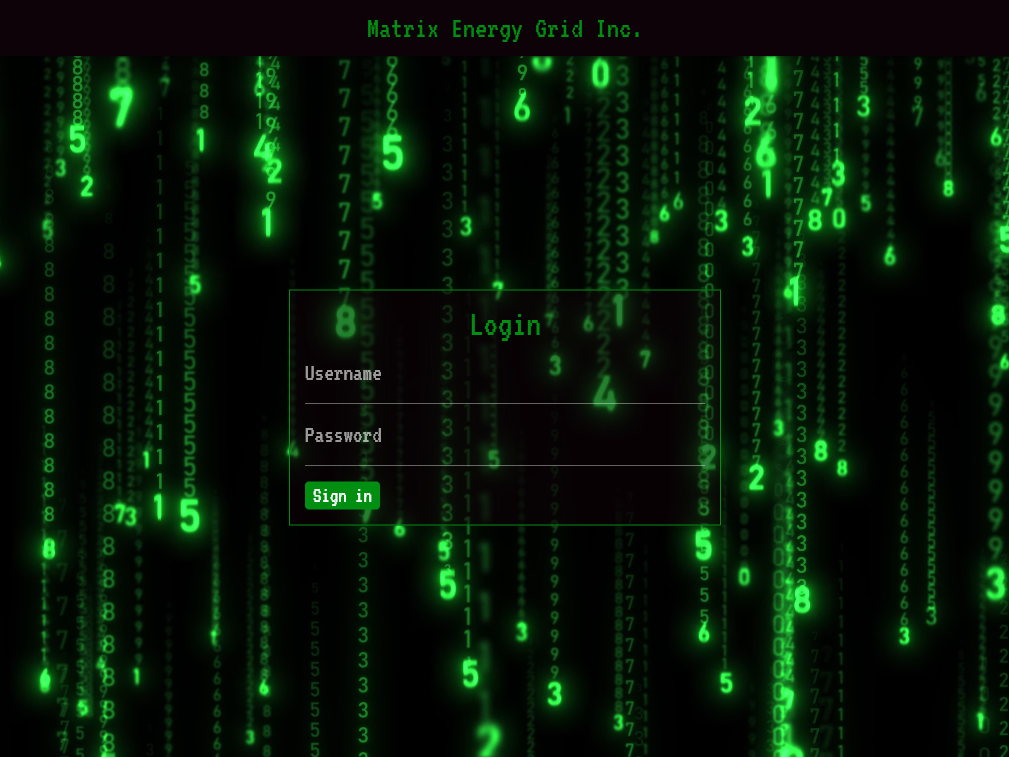
\includegraphics[width=.7\textwidth]{img/login.png}
    \caption{Anmeldebildschirm unter Port 80}
\end{figure}

Es gibt mehrere Möglichkeiten, an die Zugangsdaten zu gelangen. Der einfachste Weg wäre, einen Blick auf den HTML-Quelltext der Website zu werfen, welcher \blockquote{Test-Zugangsdaten} enthält oder einen Bruteforce-Angriff durchzuführen, welcher dadurch erleichtert wird, dass das Backend in der Rückmeldung angibt, ob Passwort oder Benutzername falsch waren, und sowohl Benutzername als auch Passwort weit oben in der \texttt{rockyou.txt} erscheinen.

\begin{lstlisting}[language=HTML]
<!DOCTYPE html>
<!--
FOR TESTING ONLY!!!
Credentials:
Username: smithy
Password: 010101
-->

<html>
\end{lstlisting}

Nach der Eingabe der Zugangsdaten aus dem HTML-Quelltext erhält man Zugriff auf die Verwaltungsoberfläche der \enquote{Matrix Energy Grid Inc.}


\begin{figure}[!ht]
    \centering
    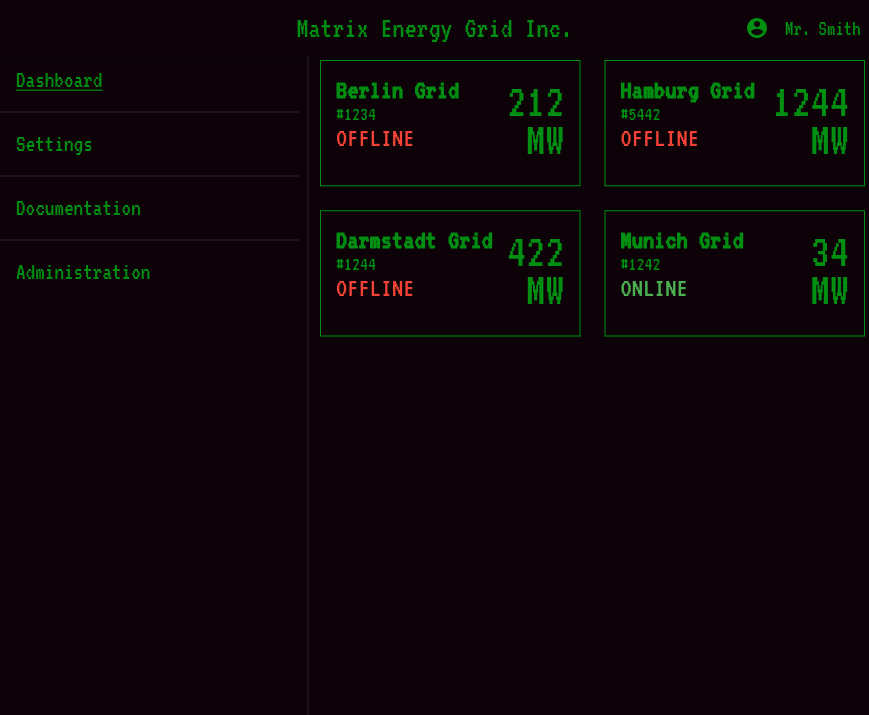
\includegraphics[width=.7\textwidth]{img/dashboard.png}
    \caption{Dashboard nach der Anmeldung}
\end{figure}

Unter dem Menüpunkt \blockquote{Settings} können nun Profilinformationen abgerufen werden. Dabei lässt sich feststellen, dass der eingeloggte Benutzer keine Administratorrechte hat. Ferner erlaubt die Seite die Änderung des Anzeigenamens.

\begin{wrapfigure}{r}{0.5\textwidth}
    \centering
    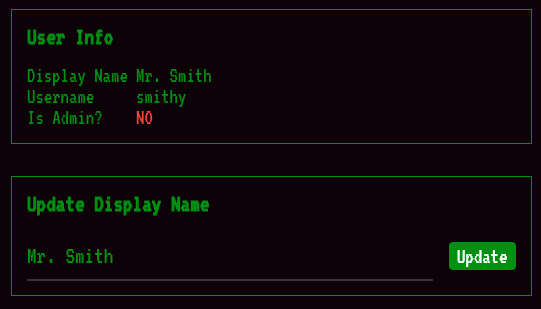
\includegraphics[width=.5\textwidth]{img/settings.png}
    \caption{Profileinstellungen}
\end{wrapfigure}

Das Verfahren zur Sitzungsverwaltung sieht zunächst sicher aus:
Angelehnt an JSON~Web~Tokens~(JWT) wird vom Server eine Payload-JSON generiert, die die Profilinformationen enthält.
Diese Payload wird über einen HMAC mit einem geheimen \texttt{SECRET} signiert und die Signatur dann anschließend zusammen mit der Payload als base64 in einem Cookie \texttt{MATRIXSESSION} gespeichert.
Bei weiteren Anfragen sendet der Browser den Cookie, und der Server überprüft nur die Signatur und kann vertrauen, dass die Profilinformationen in der Payload korrekt sind -- die Payload wurde schließlich vom Server selbst ausgestellt.
Der Signaturalgorithmus wird in der API-Dokumentation, die ebenfalls über die Webseite gelesen werden kann, beschrieben.

Mit der Implementierung eines eigenen kryptographischen Protokolls hat sich jedoch eine Schwachstelle aufgetan:
Für den HMAC wurde bcrypt als Hashfunktion verwendet.
Jedoch kann bcrypt Eingaben, die länger als 72~Bytes sind, nicht verarbeiten; überstehende Bytes werden ignoriert.
Effektiv deckt die Signatur also nur die ersten $(\hbox{72} - \hbox{\textit{Länge des \texttt{SECRET}}})$ Zeichen der Payload ab, die verbleibenen Zeichen können jedoch durch den Angreifer modifiziert werden, ohne dass die Signatur invalidiert wird.

Ein \texttt{MATRIXSESSION}-Cookie kann etwa wie folgt aussehen:
\begin{lstlisting}
eyJ1c2VybmFtZSI6InNtaXRoeSIsImRpc3BsYXlfbmFtZSI6Ik1yLiBTbWl0aCIsImlzX2FkbWluIjpmYWxzZX0=.JDJhJDEwJGs0OWcxL21ONTFUVUcuUmxlUnVvbnVNTmY2NHNEekJVVWx1dXBrZ25hUnJhdkZYTmFuWDNH
\end{lstlisting}

Rechts vom Punkt befindet sich der HMAC, links vom Punkt die Payload.
Diese dekodiert zu
\begin{lstlisting}[language=JSON]
{"username":"smithy","display_name":"Mr. Smith","is_admin":false}
\end{lstlisting}

\begin{wrapfigure}{r}{0.5\textwidth}
    \centering
    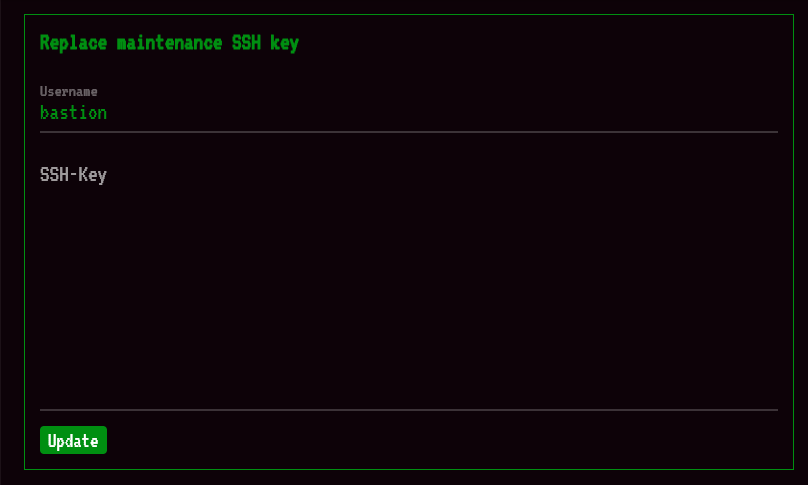
\includegraphics[width=.5\textwidth]{img/ssh.png}
    \caption{Hochladen des SSH-Key}
\end{wrapfigure}

Das Flag \texttt{is\_admin} ist der letzte Eintrag in der JSON.
Gelingt es also, zusammen mit dem unbekannten \texttt{SECRET} mindestens 72~Zeichen vor dem \texttt{false} einzufügen, dann wird diese Flag nicht von der Signatur abgedeckt und kann somit beliebig manipuliert werden.

Tatsächlich kann der \texttt{display\_name} über die Profileinstellungen geändert werden.
Das Frontend begrenzt zwar die Länge des Anzeigenamens, das Backend allerdings nicht.
So kann man einen neuen Cookie bekommen, bei dem ein entsprechend langer \texttt{display\_name} dafür sorgt, dass die Signatur eine Änderung von \texttt{is\_admin} auf \texttt{true} erlaubt.
Mit dem Admincookie erlangt man nun Zugriff auf das Admin-Panel, über das ein SSH-Key für den \texttt{bastion}-Linux-User hochgeladen werden kann.
Nach dem Login über SSH erscheint das erste Token in der Message~of~the~day:
\lstinputlisting{tokens/token1}
